\section{Resilienz- und Fehlertoleranzstrategien}


Verschiedene Strategien und Konzepte, wie Redundanz, Partitionierung und Skalierbarkeit,
bieten Ansätze, um Systeme robust und flexibel zu gestalten.

\subsection{Redundanz}

Redundanz bezeichnet in technischen Systemen die bewusste Vervielfältigung kritischer Komponenten oder Funktionen,
um die Zuverlässigkeit und Verfügbarkeit des Gesamtsystems zu erhöhen.
Durch diese Mehrfachauslegung kann das System trotz des Ausfalls einzelner Elemente weiterhin ordnungsgemäß
funktionieren.
Dieses Prinzip findet insbesondere in sicherheitskritischen Bereichen Anwendung, um die Ausfallsicherheit
zu gewährleisten.
Man unterscheidet dabei zwischen den Konzepten der aktiven und passiven Redundanz, die als Architekturdesigns
betrachtet werden können, sowie zwischen verschiedenen technischen Implementierungsebenen der Redundanz wie Software-,
Hardware-, Daten-, Netzwerk- und geografischer Redundanz.

\paragraph{Aktive Redundanz}
In dieser Art von Redundanz arbeiten mehrere Komponenten gleichzeitig und parallel, um dieselbe Funktion auszuführen.
Falls eine der Komponenten ausfällt, übernehmen die verbleibenden Einheiten ihre Aufgaben nahtlos, ohne Unterbrechungen
oder Leistungseinbußen.

\paragraph{Passive Redundanz}
Hier bleibt die redundante Komponente in einem Standby-Zustand und wird erst aktiviert, wenn die primäre Komponente ausfällt.
Im Gegensatz zur aktiven Redundanz benötigt dieser Ansatz eine kurze Umschaltzeit, um die redundante Komponente in
Betrieb zu nehmen.

Während aktive und passive Redundanzen die Vorgehensweise festlegen, wie Redundanz in einem System genutzt wird,
konzentrieren sich die technischen Implementierungsebenen darauf, welche Elemente redundant sind und auf welcher Ebene
die Redundanz umgesetzt wird.


\paragraph{Software-Redundanz} bezieht sich auf die Implementierung mehrerer gleichwertiger oder ergänzender
Softwarekomponenten, die dieselbe Funktionalität erfüllen können.
Dies wird häufig genutzt, um Softwarefehler oder Programmabstürze abzufangen.
Ein Beispiel ist das Design redundanter Algorithmen oder die Verwendung von \enquote{N-Version Programming}, bei
dem verschiedene Softwareversionen unabhängig voneinander entwickelt und parallel ausgeführt werden.
\paragraph{Hardware-Redundanz} beschreibt die Mehrfachvorhandenheit physischer Komponenten in einem System, um
dessen Zuverlässigkeit zu erhöhen.
Typische Beispiele sind Redundanz in Form von doppelten Netzteilen, CPUs oder Festplatten.
RAID-Systeme (Redundant Array of Independent Disks) verwenden z.B.\ Hardware-Redundanz,
um Datenverluste bei einem Festplattenausfall zu verhindern.
\paragraph{Daten-Redundanz} bezieht sich auf die mehrfach vorhandene Speicherung oder Repräsentation derselben Daten.
Sie wird häufig in Datenbanksystemen oder Cloud-Umgebungen eingesetzt, um sicherzustellen, dass Daten bei einem
Systemausfall oder einer Beschädigung verfügbar bleiben.
Ein Beispiel ist die Verwendung von Datenreplikation oder Backup-Strategien, die die Daten an mehreren
Standorten oder in mehreren Versionen speichern.
\paragraph{Netzwerk-Redundanz} bezeichnet die Implementierung alternativer Datenübertragungswege und -ressourcen,
um sicherzustellen, dass Kommunikationsnetzwerke auch bei einem Ausfall einer Verbindung oder eines Knotens
funktionsfähig bleiben.
Typische Methoden umfassen redundante Switches, Router oder Glasfaserverbindungen.
\paragraph{Geografische Redundanz} beschreibt die Verteilung von Systemressourcen und Daten an mehreren geografisch
getrennten Standorten.
Dieses Konzept wird verwendet, um die Auswirkungen von Naturkatastrophen, Stromausfällen oder
anderen großflächigen Störungen zu minimieren~\cite{g4g-redundancy}.


%Literature:
%https://www.geeksforgeeks.org/redundancy-system-design/

\subsection{Partitionierung}

Partitionierung bezeichnet den Prozess der physischen Unterteilung von Daten in kleinere, logisch zusammenhängende
Einheiten (Partitionen), die unabhängig voneinander verwaltet und abgerufen werden können.
Dieses Konzept wird verwendet, um die Skalierbarkeit zu verbessern, die Leistung zu optimieren, Konflikte
bei Datenzugriffen zu reduzieren und mehr Flexibilität im Umgang mit Daten zu schaffen.
Partitionierung ist insbesondere in umfangreichen Datenlösungen von Bedeutung, da sie es ermöglicht,
Daten effizient zu organisieren und auf spezifische Nutzungsmuster abzustimmen.

\begin{figure}[t]
  \centering
  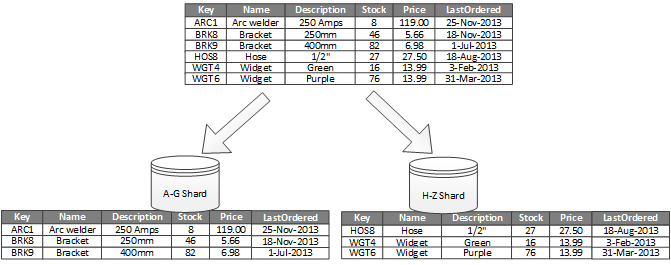
\includegraphics[width=\linewidth]{../images/1}
  \caption{Horizontale Partitionierung~\cite{mic-datapar}}
    \label{fig:datapar}
  \Description{Eine Datenbanktabelle wird horizontal skaliert: Shards mit Schlüssel A-G auf einer Tabelle, H-Z auf einer anderen}
\end{figure}

\paragraph{Die horizontale Partitionierung} unterteilt Datensätze einer Tabelle in mehrere Partitionen,
wobei jede Partition eine Untermenge der Gesamtdaten darstellt.
Dies geschieht auf der Grundlage eines Partitionsschlüssels, der dazu dient, die Daten gleichmäßig zu verteilen.
Jede Partition kann unabhängig gespeichert und verwaltet werden, wodurch eine hohe Skalierbarkeit und
Lastverteilung gewährleistet wird.
Diese Methode reduziert Konflikte bei gleichzeitigen Datenzugriffen und ist besonders nützlich in groß angelegten,
verteilten Systemen.
\paragraph{Die vertikale Partitionierung} teilt eine Tabelle in mehrere Partitionen,
indem sie Spalten oder Attribute gruppiert.
Häufig verwendete Attribute werden in einer Partition gespeichert, während weniger relevante oder selten genutzte
Attribute in separaten Partitionen abgelegt werden.
Diese Strategie optimiert die Leistung, weil Abfragen nur auf die relevanten Daten zugreifen müssen.
\paragraph{Die funktionale Partitionierung} organisiert Daten basierend auf ihrer Funktion oder ihrem Zweck
innerhalb eines Systems.
Unterschiedliche logische Datensätze werden in separaten Partitionen abgelegt, die unabhängig voneinander verwaltet
werden können.
\paragraph{Die RANGE-Partitionierung} teilt Daten anhand von Wertebereichen auf.
Diese können auf numerischen, zeitlichen oder anderen skalierbaren Kriterien basieren.
Diese Methode erleichtert die Organisation und Verwaltung der Daten erheblich.
Besonders bei regelmäßigen Archivierungs- oder Löschvorgängen ist die Verwaltung von Bereichspartitionen vorteilhaft,
da Partitionen eigenständig bearbeitet werden können.
\paragraph{Die HASH-basierte Partitionierung} verwendet eine Hash-Funktion, um Daten basierend auf einem bestimmten
Feld auf Partitionen zu verteilen.
Diese Methode sorgt für eine gleichmäßige Verteilung der Daten und verhindert die Entstehung von Hotspots.
Sie eignet sich besonders für Systeme, die eine gleichmäßige Workload-Verteilung und optimale Ressourcennutzung erfordern.
\paragraph{Die Round-Robin Partitioning} verteilt Daten in zyklischer Reihenfolge gleichmäßig auf alle verfügbaren Partitionen.
Sie ist eine einfache und leicht implementierbare Methode, um eine gleichmäßige Verteilung der Daten zu gewährleisten.
Diese Strategie ist jedoch weniger effizient bei datenabhängigen Abfragen,
da Daten nicht nach logischen Gruppen organisiert sind~\cite{g4g-partitioning}.

%Literature:
%https://learn.microsoft.com/de-de/azure/architecture/best-practices/data-partitioning

%Literature:
%https://www.geeksforgeeks.org/data-partitioning-techniques/

\subsection{Skalierbarkeit}

Skalierbarkeit bezeichnet die Fähigkeit eines Systems, seine Ressourcen und Kapazitäten flexibel an
veränderte Anforderungen anzupassen, wie etwa wachsende Nutzerzahlen, größere Datenmengen oder eine erhöhte Verarbeitungslast.
Dieses Prinzip ist entscheidend, um Systeme zukunftssicher zu gestalten und sowohl kurzfristige Spitzenbelastungen als auch
langfristiges Wachstum effizient zu bewältigen.
Skalierbarkeit wird dabei in zwei grundlegende Ansätze unterteilt:


\paragraph{Vertikale Skalierung (Scale Up)} umfasst die Erweiterung der Ressourcen eines einzelnen Systems, um dessen
Kapazität zu steigern.
Dabei werden die Hardware-Komponenten, wie Prozessoren, Arbeitsspeicher oder Speicherplatz, aufgerüstet,
um eine höhere Leistung zu erzielen.
Vertikale Skalierung bezieht sich ausschließlich auf die Verbesserung eines einzigen Servers oder einer
einzelnen Instanz, ohne zusätzliche Systeme hinzuzufügen.
Diese Methode basiert auf der Optimierung bestehender Ressourcen innerhalb einer zentralen Einheit.
\paragraph{Horizontale Skalierung (Scale Out)} erweitert die Kapazität eines Systems durch das Hinzufügen
zusätzlicher Server, Instanzen oder Knoten, die parallel arbeiten.
Sie basiert auf der Schaffung eines verteilten Systems, in dem Arbeitslasten und Daten gleichmäßig
über mehrere Einheiten verteilt werden.
Bei dieser Methode bleibt die Leistung nicht auf ein einzelnes System beschränkt, da die Arbeitslast von mehreren
Ressourcen gleichzeitig bearbeitet wird.
Die horizontale Skalierung setzt eine verteilte Architektur voraus, bei der mehrere Systeme miteinander verbunden sind,
um die Gesamtleistung zu erhöhen~\cite{ibm-scaling}.
\paragraph{Automatische Skalierung} ist der Prozess, bei dem Ressourcen dynamisch und flexibel an die aktuellen
Leistungsanforderungen einer Anwendung angepasst werden.
Automatische Skalierung wird häufig in Cloud-Umgebungen eingesetzt, bei denen Ressourcen automatisch hinzugefügt
oder entfernt werden, abhängig von der aktuellen Last oder dem Bedarf.
Dieses Konzept minimiert den manuellen Verwaltungsaufwand und stellt sicher, dass Systeme jederzeit optimal
konfiguriert sind~\cite{mic-autoscaling}.


%Literature:
%https://www.ibm.com/think/topics/scale-up-vs-scale-out
%https://azure.microsoft.com/en-us/resources/cloud-computing-dictionary/scaling-out-vs-scaling-up
